% -*- LaTeX -*-
% -*- coding: utf-8 -*-
%
% michael a.g. aïvázis
% orthologue
% (c) 1998-2018 all rights reserved
%

%-----------------------------------

\section{applications}

% --------------------------------------
% the application harness
\begin{frame}[fragile]
%
  \frametitle{Creating an application}
%
  \vskip -3ex
  \begin{itemize}
%
  \item applications are the top level component managers
%
    \python{firstnumber=10,linerange={10-34}}{listings/quad.py}
%
  \end{itemize}
%
\end{frame}

% --------------------------------------
% the application harness
\begin{frame}[fragile]
%
  \frametitle{Auto-launching}
%
  \begin{itemize}
%
  \item instantiating and launching the application
%
    \python{firstnumber=54,linerange={54-60}}{listings/quad.py}
%
  \item a sample configuration file
%
    \cfg{firstnumber=8, linerange={8-20}}{listings/quad.cfg}
%
  \end{itemize}
%
\end{frame}

% --------------------------------------
% the application component
\begin{frame}[fragile]
%
  \frametitle{The application component}
%
  \begin{itemize}
%
  \item the shell hierarchy in pyre
%
  \begin{figure}
    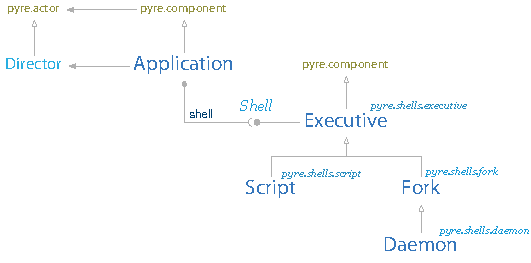
\includegraphics[scale=1.0]{figures/shells.pdf}
  \end{figure}
%
  \item our \identifier{Quad} derives from \identifier{Application}, so it has a
    \identifier{shell}
%
  \end{itemize}
%
\end{frame}

% --------------------------------------
% the parallel version
\begin{frame}[fragile]
%
  \frametitle{Parallel integration}
%
  \begin{itemize}
%
  \item the \identifier{mpi} entry point
%
    \python{firstnumber=36,linerange={36-52}}{listings/quad.py}
%
  \item the \package{mpi} package is part of the pyre distribution
    \begin{itemize}
    \item handles initialization and finalization of \package{MPI}
    \item simplifies most of the ``overhead'' activities
    \item provides an OO veneer
    \end{itemize}
%
  \end{itemize}
%
\end{frame}

% --------------------------------------
% running the mpi program
\begin{frame}[fragile]
%
  \frametitle{Running in parallel}
%
  \begin{itemize}
%
  \item minor modifications to the configuration file...
%
    \cfg{firstnumber=8, linerange={8-28}}{listings/quad.cfg}
%
  \end{itemize}
%
\end{frame}

%-----------------------------------
% end of file
